\chapter{Introduction} 
\label{chapter-intro} 

% 1. have a narrative!! 
% 2. make it absolutely clear that no one has done it before AND we have to figure this out!!

\section{Motivation and significance}
\label{intro-motivation}
In vision science, core object recognition has largely been modeled as a feed-forward process down the visual ventral stream \cite{dicarlo_how_2012}. First of such feed-forward models was Hubel and Wiesel's hierarchy model \cite{hubel_receptive_1962}, which classified the neurons in the visual cortex into simple and complex cells. This idea directly inspired the Neocognitron model \cite{fukushima_neocognitron_1980}, which in turn provided the basis for Convolutional Neural Networks (CNNs) \cite{alexnet},\cite{lenet}, which have become a dominant model in computer vision \cite{yamashita_convolutional_2018}. However, recent research starts to suggest that these feed-forward neural networks fail to model various key features in early primate vision  \cite{oreilly_recurrent_2013}, \cite{spoerer_recurrent_2017}, \cite{ricci_same-different_2018}, \cite{kietzmann_recurrence_2019}, \cite{van_bergen_going_2020}. In addition, across the different stages of early visual processing, the nature of neural computations vary drastically, particularly between the retina and the primary visual cortex (V1) \cite{dyballa_manifold_2021}. 

To this end, we seek to investigate the following related open questions:
\begin{itemize}[noitemsep, topsep=0pt]
    \item How do computer vision (CV) models (VGG16 \cite{vgg16_simonyan_very_2015}, Vision Transformer \cite{vit_dosovitskiy_image_2021}, and Convolutional Recurrent Neural Network \cite{convrnn_shi_end--end_2015}) compare to biological vision, at retina and primary visual cortex (V1), in terms of their respective neural circuits\footnote{A neural circuit is a population of neurons interconnected by synapses to carry out a specific function when activated \cite{gerhard_neuroscience_2013}.}?
     
    \item What specific mechanisms are important in causing such differences and/or similarities?
\end{itemize}

\begin{figure}[H]
\centering
\begin{subfigure}[b]{0.5\textwidth}
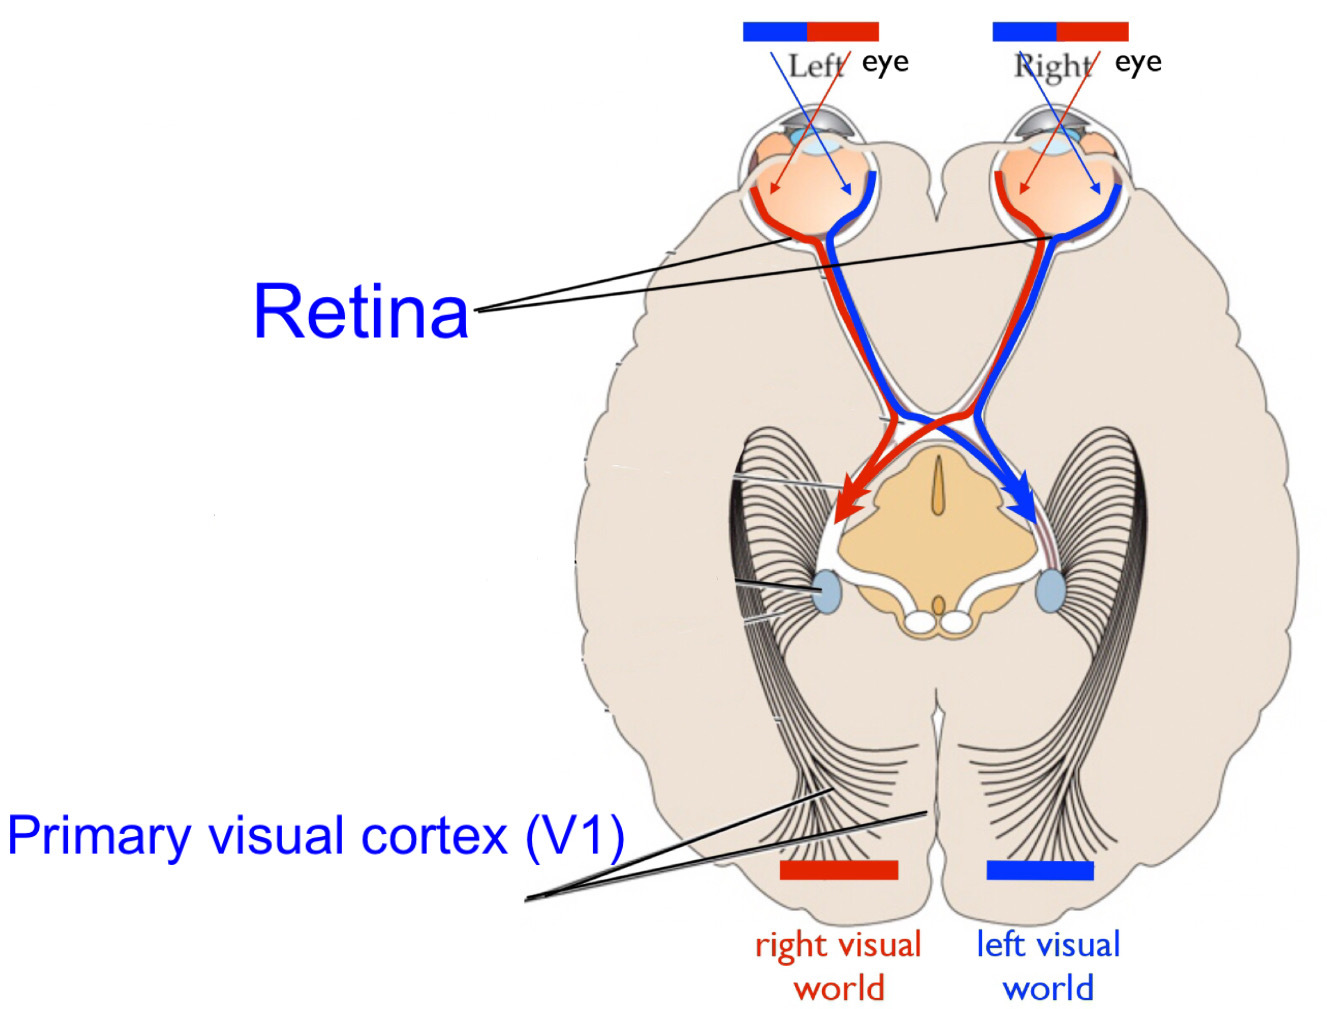
\includegraphics[width=\textwidth]{figures/intro/visual-pathway.jpg}
    \caption{Early visual pathway (from retina to LGN to V1). Adapted from \cite{pillow_vision_2022}}
\end{subfigure}
\hfill
\begin{subfigure}[b]{0.45\textwidth}
      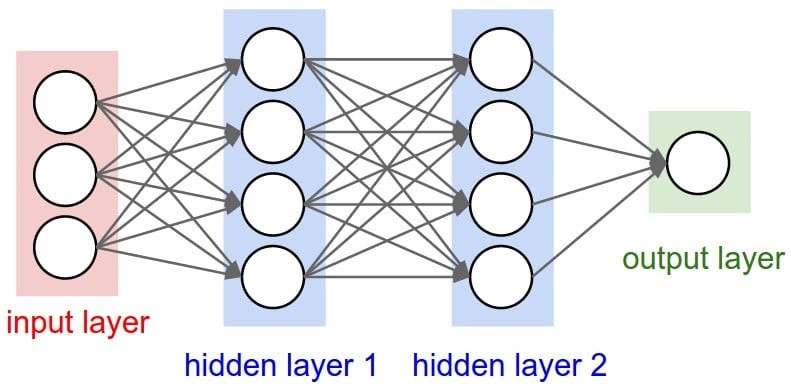
\includegraphics[width=\textwidth]{figures/intro/simple-ann.jpeg}
    \caption{Illustration for a simple ANN with two hidden layers.}
\end{subfigure}
\end{figure} 

\par The significance of answering these questions is two-fold. First, modeling the visual system has always been an important task in the field of neuroscience. Despite decades of research, we have not fully understood the structure of neural circuits responsible for visual perception \cite{Gwilliams221630}. Second, for the computer vision community, in addition to the existing research on explainability of computer vision models, there is a growing interest in investigating the limitations of these models by comparing them against biological vision. A growing number of research starts to reveal tasks that biological vision excels at while the state-of-the-art computer vision models fail. One notable example is that CNN is highly inferior to human vision in solving visual problems that involve relational reasoning \cite{glorot-bengio-difficulty}, such as recognizing same-different relations in images \cite{ricci_same-different_2018}, categorizing images based on the constituent parts \cite{visual-categorization}, and comparing features in images  \cite{cnn-human-abstraction}. The hope is that with a rigorous comparison, we can discover the specific mechanisms responsible for certain desired features of biological vision that the current computer vision models are lacking and adapt those mechanisms into computer vision models with relevant computational constraints in mind.
% Some of the concrete examples of recent breakthroughs in computer vision that takes inspiration from biological vision are reviewed in section \ref{brain-inspired}. 

% ([to-do] Specific to our project, why would computer vision models learn from biological vision? what is the advantage? does recurrence helps vision??)

% In the field of AI, more sophisticated models of the visual system could inspire new computational algorithms in solving increasingly demanding computer vision tasks. In fact, research in computer vision has taken many inspirations from neuroscience. In LeCun, Bengio, \& Hinton's seminal work on deep learning (\cite{lecun_deep_2015}), they stated that ``ConvNets have their roots in the Neocognitron," which was one of the earliest computational models of the visual system. 
\section{Framework of comparison}
\label{intro-framework}
Both subjects of our study, artificial and biological neural networks, are instances of black box problem where the underlying function is unknown. The best approach to investigate the internal structure of a black box system is to probe the system with some input and record the output:
\begin{figure}[H]
    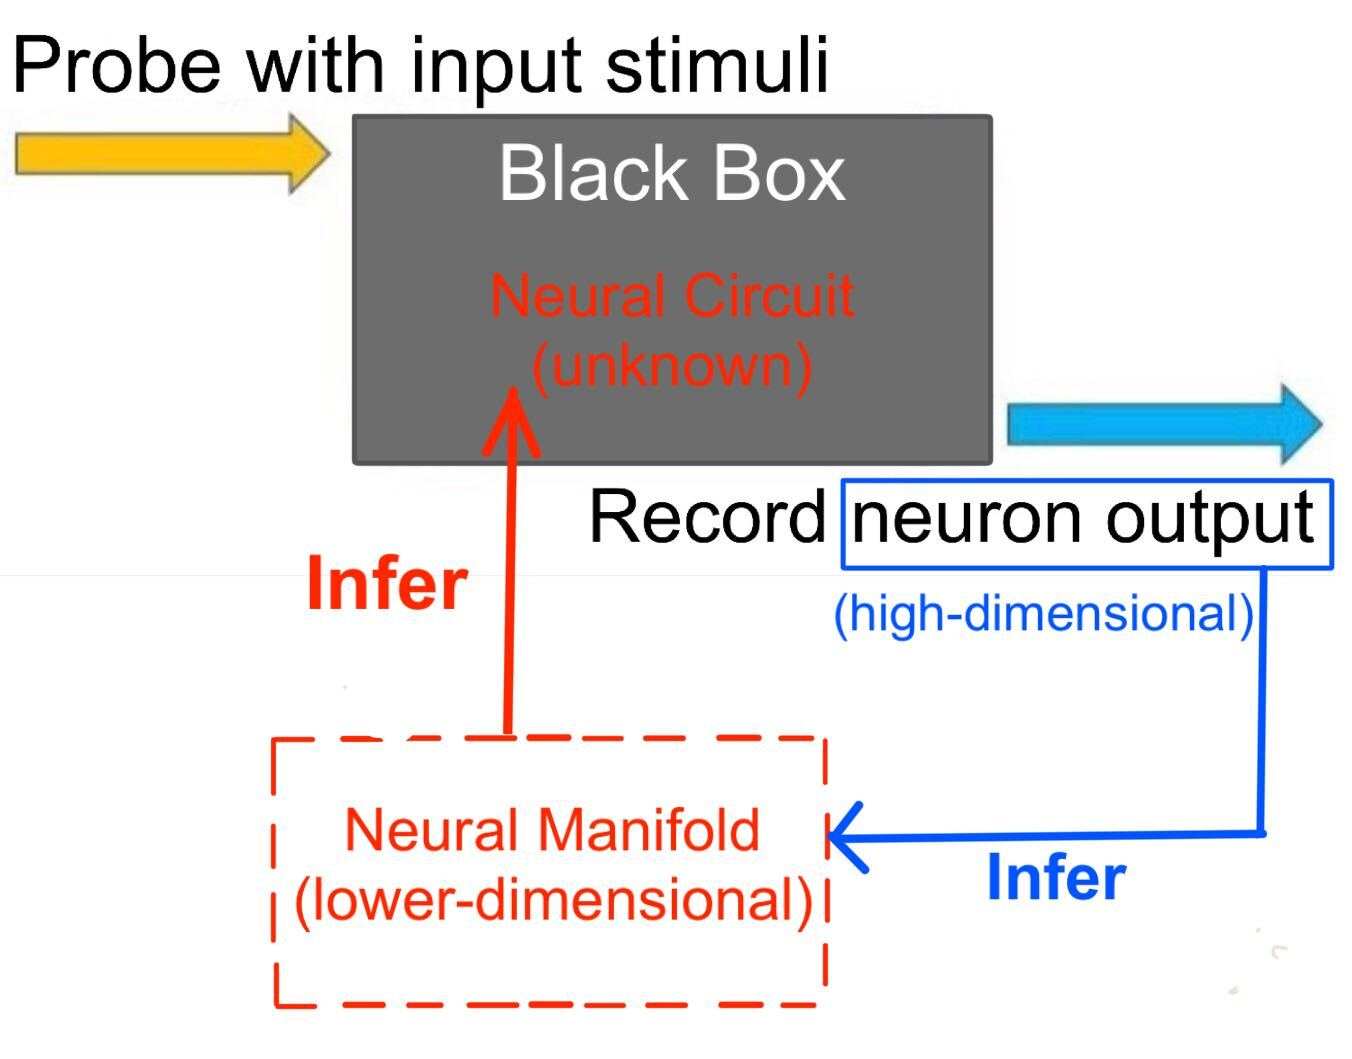
\includegraphics[width=0.85\textwidth]{figures/intro/black-box.jpg}
    \caption{Illustration of the black box problem.}
\end{figure} 

Applying this approach to our problem, we compare the neural circuits of artificial and biological neural networks (both unknown \textit{a priori}) by comparing the neural output from each network when given the appropriate input. Since the neural output is encoded in high-dimensional representations, it is impossible to analyze the organization of neurons directly based on their responses to visual stimuli. For this reason, we need to infer an intermediate lower-dimensional representation, which we call ``neural manifold" and will be our basis for comparison. 

\subsection{ \textit{What is a neural manifold?}}
\par In order to formalize the concept of neural manifold, we first introduce the definition of a manifold as a mathematical object.

\begin{defn}[Homeomorphism]
Let $f: X \to Y$ be a function between topological spaces $X$ and $Y$. If $f$ is bijective, then the inverse $f^{-1}$ exists. If both $f$ and $f^{-1}$ are continuous, then $f$ is a \underline{homeomorphism}. The two topological spaces, $X$ and $Y$, are said to be \underline{homeomorphic} if there exists a homeomorphism between $X$ and $Y$. 
\end{defn}
    \begin{defn}[Manifold]
   In brief, a \underline{real $n$-dimensional manifold} is a topological space $\mathcal{M}$ for which every point $x\in\mathcal{M}$ has a neighborhood homeomorphic to Euclidean space $\RR^n$. Informally, a manifold is a topological space that locally resembles Euclidean space.
    \end{defn}
   \begin{figure}[H]
      \centering
     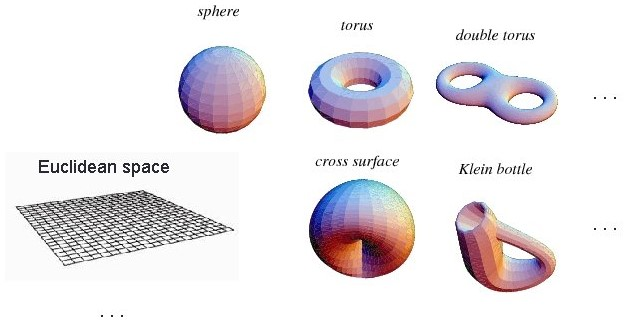
\includegraphics[width=0.4\textwidth]{figures/intro/manifold.jpg}
     \caption{Examples of $2$-dimensional manifolds.}
    \end{figure} 
            
Formally, the neural manifold is a lower-dimensional topological space embedded in the high-dimensional Euclidean space where the original neural output belongs. Why is the neural manifold still a good representation of the organization of neurons even if it is of a lower dimension?  The general justification rests on ``the Manifold Hypothesis\footnote{the Manifold Hypothesis forms the basis of a collection of methods called Manifold Learning}," which states that naturally occurring data form lower-dimensional manifolds in the embedding space \cite{colah-manifold}. The neuroscientific justification is based on the established fact that despite the original high-dimensional representations, the possible patterns of neural output are confined to a lower-dimensional manifold spanned by a few independent patterns called ``neural modes"  \cite{gallego_neural_2017}, \cite{stopfer_intensity_2003}, \cite{yu_gaussian-process_2009}.

% In other words, the number of variables that are really necessary to describe the data is much smaller than the number of variables in the original representation.
\begin{rmk}
For ease of reference, we also use the term ``neural manifold" for the point-cloud of data points with an underlying manifold structure. In addition, neural manifolds from real neural data are often no longer ``manifolds” in a mathematical sense, due to the sparse input sampling and the presence of neural noise. 
\end{rmk}

\subsection{\textit{What can we analyze from a neural manifold?}}
\label{intro-network-manifold}
Neural manifold is an intermediate step from the neural output towards inferring the neural circuits. On the neural manifold, each point represents a neuron. The distance between a pair of points indicates how similar the firing patterns of the corresponding neurons are, and equivalently, how likely they participate in the same neural circuit. To infer the (unknown) neural circuit from a neural manifold (known), we note that there are three possible cases: if neurons were originally sampled 
\begin{enumerate}[noitemsep,topsep=0pt]
    \item from a collection of isolated neural circuits (decomposable networks), then the neurons would have distinct stimuli preferences, yielding a discontinuous neural manifold.
    \item from overlapping neural circuits (partially decomposable networks), most neurons would respond to multiple stimuli, leading to a smooth transition in stimuli preferences and a continuous neural manifold. 
    \item from fully connected neural circuits (non-decomposable networks),  all neurons would respond to all stimuli, and there would be no stimuli preferences across groups of neurons. This would yield a zero-dimensional (i.e., degenerate) manifold.
\end{enumerate}

\begin{figure}[H]
\label{networks-manifolds}
\centering
    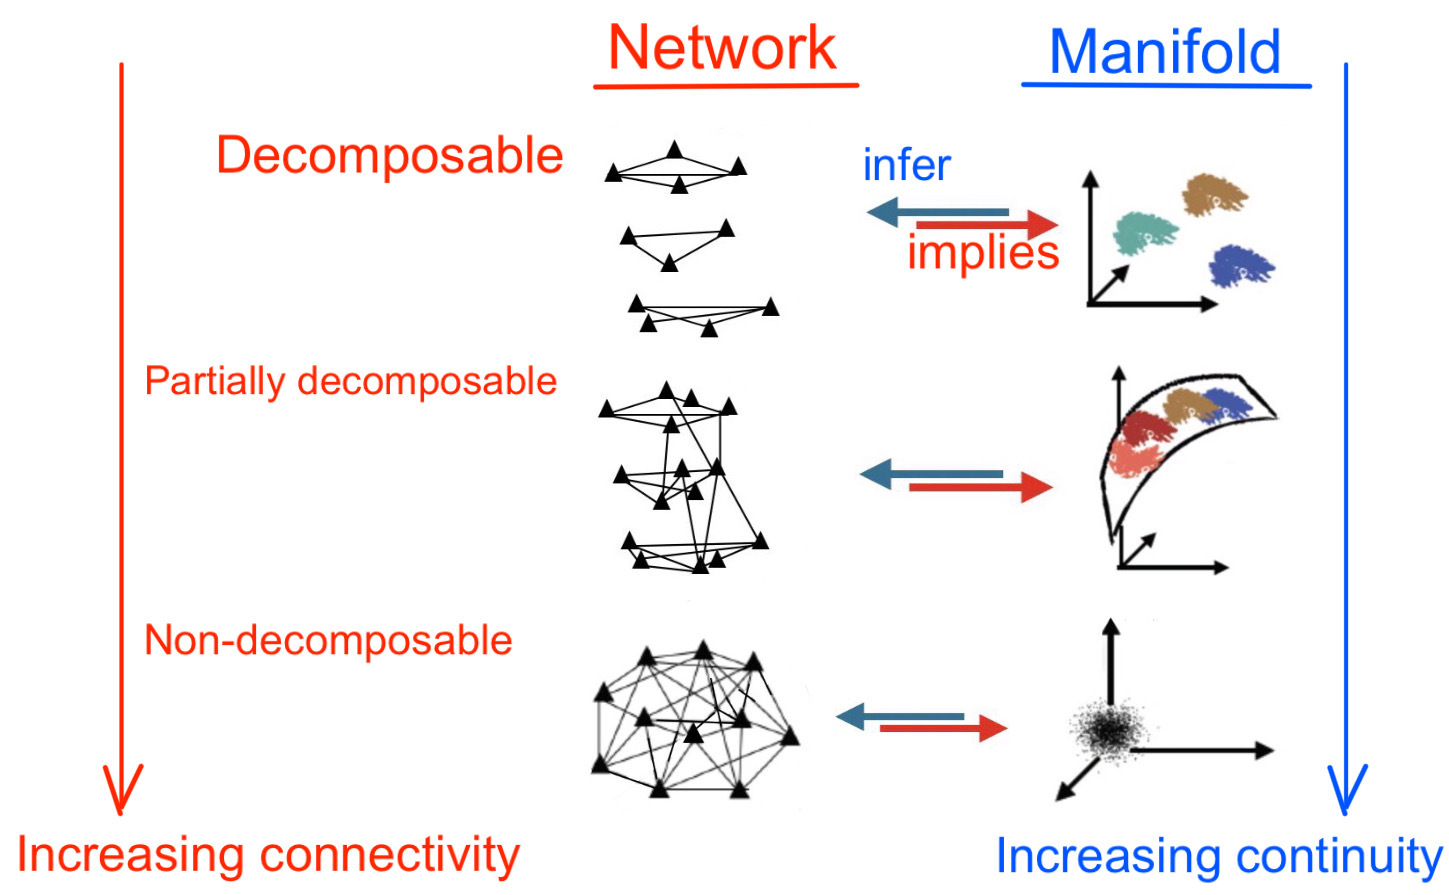
\includegraphics[width=0.55\textwidth]{figures/intro/networks-manifolds.jpg}
    \caption{Connections between neural manifolds and neural circuits. Adapted from \cite{dyballa_manifold_2021}.}
\end{figure} 
To sum up, by comparing the continuity of neural manifolds arising from artificial and biological neural networks, we can make precise inferences about their similarities and differences of their respective neural circuits, which is what we set out to compare in \ref{intro-motivation}.


\section{Problem statement}
\label{intro-objective}

Our starting point was the result in \cite{dyballa_manifold_2021}: based on the respective neural manifolds, the retinal ganglion cells differ fundamentally from the functional cells in V1 which are distributed more continuously. 
% \begin{figure}[H]
% \centering
% \begin{subfigure}[b]{0.5\textwidth}
%             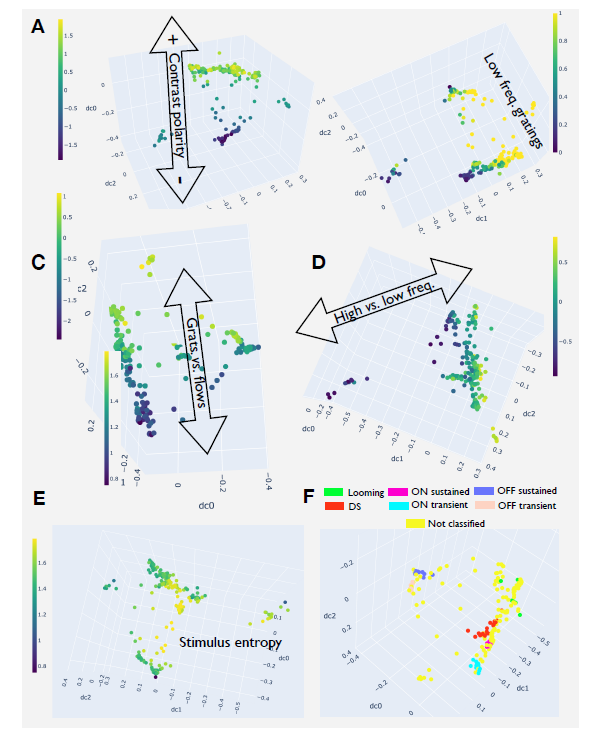
\includegraphics[width=0.6\textwidth]{figures/embeddings/retina-manifold.PNG}
%             \caption{Retina neural manifold (discontinuous).}
% \end{subfigure}
% \hfill
% \begin{subfigure}[b]{0.4\textwidth}  
%       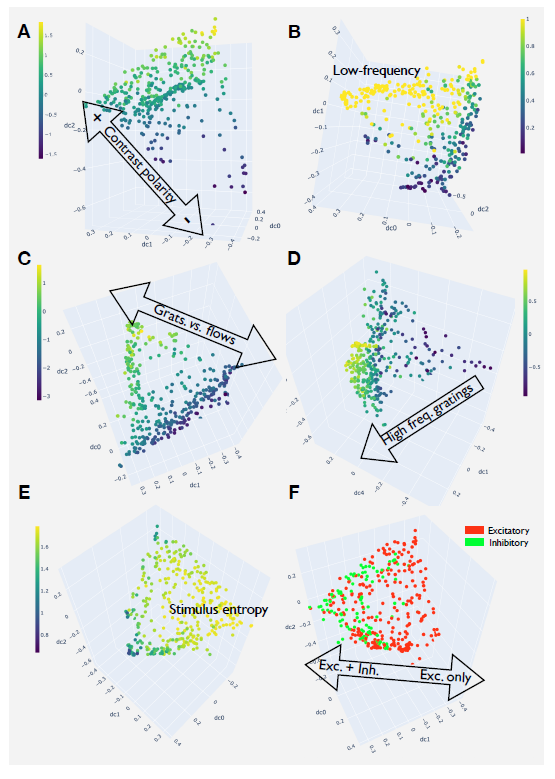
\includegraphics[width=0.6\textwidth]{figures/embeddings/v1-manifold.PNG}
%       \caption{V1 neural manifold (continuous).}
% \end{subfigure}

% \end{figure}     

Therefore, our objective, stated in concrete terms, is to find out among the computer vision models, which yield continuous neural manifold like V1 and which yield discontinuous neural manifold like the retina. The candidate models are CNN, Vision Transformer (ViT), and Recurrent Neural Networks (RNN), and their respective input and output are summarized in the following table.

\begin{table}[H]
\centering
\begin{tabular}{|l|l|l|}
\hline
        & Biological & Artificial     \\ \hline
Models   & retina, V1      & CNN, ViT, RNN \\\hline
Input & flow stimuli \cite{visual-flow}  & ImageNet images \cite{deng2009imagenet} \\ \hline
Output & single-neuron recording & artificial neuron output \\ \hline
\end{tabular}
\caption{Summary of comparison.} 
\end{table} 

% Building on our starting point, we obtained some original results, which can be summarized in the following conjectures to be further tested and confirmed:

% \textbf{Conjecture 1.} The manifold structure in feed-forward networks, including CNN and ViT, give rise to discontinuous neural manifold that is closer to that in retina than that in V1.

% \textbf{Conjecture 2.} Adding recurrent structure to the networks makes the manifold structure more continuous.

% justifications for doing comparison this way:
% why comparing with computer vision models?
% why choose continuity of manifold as the basis for comparison
% a good proxy for what kind of computation give rise to a continuous manifold

% basis of comparison: continuity of manifold this shows us the functional connections

% the models: CNN (convolution), RNN (recurrence), ViT (self-attention)

% By comparing the manifold structures of biological and artificial neural networks we can make precise inferences about similarities and differences in their respective functional circuits.

% conclusion: not convolution, not self-attention, but recurrence
\section{Highlights and thesis organization}

During the project, we have made the following original contributions:
\begin{enumerate}[noitemsep, topsep=0pt]
    \item conducted new computational experiments on neural data in the retina,
    \item developed an original algorithm to investigate the manifold structure of pre-trained Convolutional Neural Network (CNN) and how it evolves over the course of training,
    \item developed an original algorithm to investigate the manifold structure of pre-trained Convolutional Recurrent Neural Network (CRNN),
    \item developed an original algorithm to investigate the manifold structure of pre-trained Vision Transformer (ViT),
    \item compared and analyzed (both qualitatively and quantitatively) the manifold structure of CNN, ViT, and CRNN, against that of the neurobiological networks in retina and V1,
    \item conclusion that could advance research in both biological vision and computer vision.
\end{enumerate}

The code for this project is available at the GitHub repository\footnote{https://github.com/zhang-liu-official/capstone-liu-2022}.


The organization of the thesis follows the structure of the project in the flowchart below. After situating our work within the backdrop of related research in Chapter \ref{chapter-neuro}, we will provide the theoretical preliminaries for the linear dimensionality reduction method in Chapter \ref{chapter-linear} (its nonlinear counterpart is outlined in Appendix \ref{appendix-diffmap}). The experiments and results for biological and artificial neural networks will be elaborated in Chapters \ref{chapter-biological} and \ref{chapter-artificial} respectively. In the end, we propose the conclusion of our work and future directions. 


\vspace*{0.4cm}

\noindent\resizebox{\textwidth}{!}{\begin{tikzpicture}[font={\sf \small}]
 \def\smbwd{2cm}
  \node (BNN) at (-3.6,0.2) [draw, terminal, minimum width=\smbwd,  fill=yellow!20, minimum height=0.5cm] {Biological neural networks}; 
  \node (ANN) at (3.5,0.2) [draw, terminal, minimum width=\smbwd,  fill=yellow!20, minimum height=0.5cm] {Artificial neural networks}; 
  %------------
  \node (experimental) at (-3.6,-0.8) [draw, terminal, minimum width=\smbwd,  fill=red!20, minimum height=0.5cm]{Neural tensor (lab)};
  \node (artificial) at (3.5,-0.8)[draw, terminal,minimum width=\smbwd,  fill=red!20, minimum height=0.5cm]{Neural tensor (simulations)};
  %------------
  \node (TCA) at (0,-2)  [draw, process, minimum width=\smbwd, fill=blue!20, minimum height=0.7cm] {Dimensionality reduction (linear [Chapter \ref{chapter-linear}]; nonlinear [Appendix \ref{appendix-diffmap}])};
  %------------
  \node (biological-manifolds) at (-3.7,-3.2) [draw, terminal, minimum width=\smbwd,  fill=green!20, minimum height=0.5cm] {Neural manifold (biological) [Chapter \ref{chapter-biological}]};
  \node (artificial-manifolds) at (3.7,-3.2) [draw, terminal, minimum width=\smbwd,  fill=green!20, minimum height=0.5cm] {Neural manifold (artificial) [Chapter \ref{chapter-artificial}]};
  %------------
 \path [line](BNN) -- (experimental);
 \path [line](ANN) -- (artificial);
 \path [line](experimental) -- (TCA);
  \path [line](artificial) -- (TCA);
 \path [line](TCA) -- (biological-manifolds);
 \path [line](TCA) -- (artificial-manifolds);
 \end{tikzpicture}}
